\subsection{Semaforen}

Een semafoor is een integer die gebruikt wordt als een signaal tussen alle processen. 

Enkel 3 operaties mogen uitgevoerd worden op een semafoor:

\begin{itemize}
\item Initialize (zet de waarde van het semafoor).
\item Decrement (verlaagt de waarde van het semafoor) ook wel semWait(s) genoemd. Deze verlaagt de waarde van het semafoor met 1 en onderbreekt het proces indien het semafoor negatief wordt, totdat er een semSignal(s) wordt uitgezonden door een ander proces.
\item Increment (verhoogt de waarde van het semafoor) ook wel semSignal(s) genoemd. Deze verhoogt de waarde van het semafoor met 1 en als de waarde van het semafoor positief wordt het proces gedeblokkeerd.
\end{itemize}
\begin{figure}[htp]
    \centering
            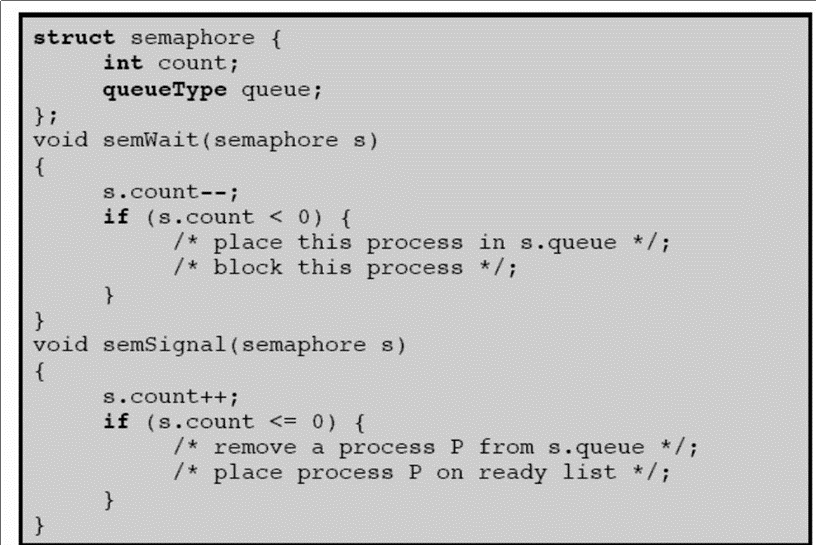
\includegraphics[width=4in]{img/semafoor.png}
        \caption{Voorbeeld van semafoor implementatie}
    \label{fig:Voorbeeld van semafoor implementatie}
\end{figure}

Een binaire semafoor kan worden geïnitialiseerd op waarde 0 of 1 en kan ook alleen maar deze twee waarden hebben.

Bewerking semWaitB() controleert waarde van de semafoor. Als de waarde nul is wordt het proces dat semWaitB() uitvoert geblokkeerd. Als de waarde 1 is wordt het proces verder uitgevoerd en de waarde in 0 veranderd.

Bewerking semSignalB() controleert of er processen op deze semafoor geblokkeerd zijn. Als dat het geval is, wordt een proces dat geblokkeerd is door een bewerking semWaitB() vrijgegeven. Zijn er geen geblokkeerde processen, waarde $\Rightarrow$ 1.

\textbf{Niet binaire semaforen worden vaak een tellende of algemene semafoor genoemd.}

Het proces dat het langst is geblokkeerd wordt als eerste vrijgelaten uit de wachtrij. Bij deze strategie is een semafoor STERK. Als de volgorde van processen uit de wachtrij niet is vastgelegd wordt het een ZWAKKE semafoor. STERKE semaforen garanderen de afwezigheid van uithongering, zwakke niet.


\subsubsection{Wederzijdse uitsluiting}

Op elk moment kan de waarde van de semafoor daarbij als volgt worden geïnterpreteerd:

\begin{itemize}
\item De waarde van de semafoor ( bij >= 0 ) is het aantal processen dat semWait(s) zonder onderbreking kan uitvoeren.
\item De waarde van de semafoor ( bij < 0 ) is het aantal processen dat is onderbroken in de wachtrij van de semafoor.
\end{itemize}


\begin{figure}[htp]
    \centering
            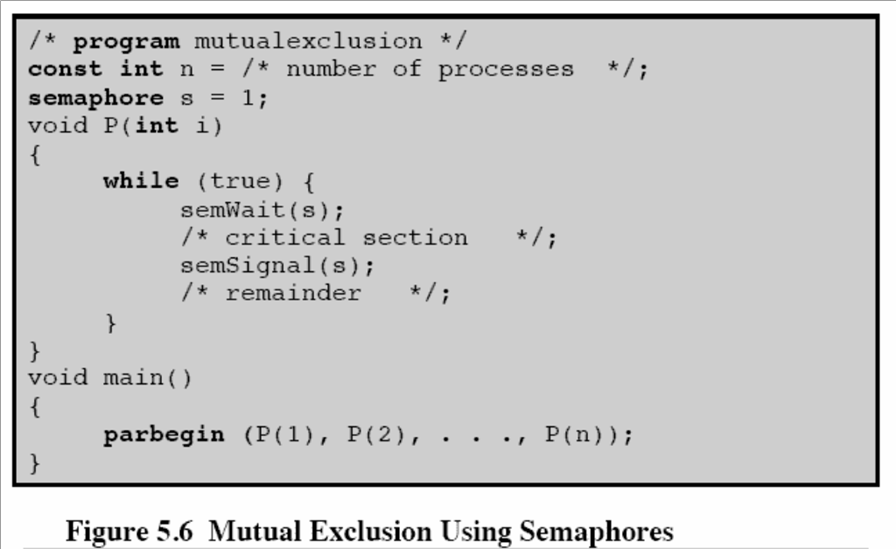
\includegraphics[width=4in]{img/mutualexclusionsemafoor.png}
        \caption{Mutual Exclusion using semaphores}
    \label{fig:Mutual Exclusion using semaphores}
\end{figure}

